\chapter{Conclusion and Future Work}
\label{conclusion}

\section{Contribution}
The contributions of this dissertation to the field of tensegrity robotics are effective state estimation from a large number of noisy senors in near real time, algorithms and methods that will control underactuated tensegrity robotic systems with limited sensor data, and implemented a control policy learned entirely through simulation with no prior knowledge of system dynamics on physical hardware.
Another smaller contribution to tensegrity robotics was the creation of the world's first unteathered underactuated tensegrity robot capable of complex controls.
Artificial neural networks (ANN) where the main control methodology used due to the inherent nonlinear system dynamics, since ANN are data driven controllers which do not require dynamic models.
Several learning methods were used to train a ANN to accomplish locomotion as well as escaping from simulated craters.
In completing these tasks, contributions were also made to the fields of machine learning and sensor fusion.

\section{Future Work}

\subsection{Re-Design of \SB{}}
\label{sec:sbv2}
\SB{} was the initial prototype for this project.
It succeeded in performing and showcasing a tensegrity robot built for locomotion, though it does have its limitations.
An evaluation of \SB{} and its limitations may be found in appendix~\ref{app:evalutation}. 

To overcome these limitations and to further expand the types of control polices for a \SB{} like robot, a re-design is proposed which has full cable actuation and will be more robust to large environmental impacts.
The largest limitation for the current design of \SB{} is the limited low level motor control, force sensing, and actuation stroke.
With the advent of robotic companies producing commercial off-the-shelf (COTS) motor solutions, using a COTS motor with integrated force sensing and control would be a viable option.
Table~\ref{cots} show a limited list of companies which offer products that could be consider for a \SB{} re-design.

% Please add the following required packages to your document preamble:
% \usepackage{graphicx}
% \usepackage[table,xcdraw]{xcolor}
% If you use beamer only pass "xcolor=table" option, i.e. \documentclass[xcolor=table]{beamer}
\begin{table}[tbhp]
\centering
\caption{List of companies that sell COTS actuators to be integrated into \SB{} v2. This is not an exhaustive list.}
\label{cots}
\resizebox{\textwidth}{!}{%
\begin{tabular}{|c|
>{\columncolor[HTML]{EFEFEF}}c |
>{\columncolor[HTML]{FFFFFF}}c |
>{\columncolor[HTML]{EFEFEF}}c |
>{\columncolor[HTML]{FFFFFF}}c |}
\hline
\textbf{Company} & Dynamixel & Kinova & Muse Robotics                                                          & Hebi Robotics \\ \hline
\textbf{Product} & MX-106    & K-58   & \begin{tabular}[c]{@{}c@{}}COTS motor \\ control boards\end{tabular} & X8-3          \\ \hline
\end{tabular}%
}
\end{table}

From table~\ref{cots}, a likely candidate to succeed is the X8-3 from Hebi Robotics.
This COTS actuator has position, velocity, and output torque control which utilizes a series elastic element to directly sense the output torque.
It also supports tunable control parameters and closed loops control parameters, which all run at \(\SI{1000}{\hertz}\) and can be tuned while the system is operating.
Thus, an initial prototype has been designed around this X8-3 motor, where single rod and end cap testing still needs to be done.
This prototype eliminates the internal springs and relies on cable stretch and motor elastic element for system passive compliance.
Figure~\ref{fig:sbv2} shows what the new design concept looks like.

\begin{figure}
\centering
\begin{subfigure}{.5\textwidth}
  \centering
  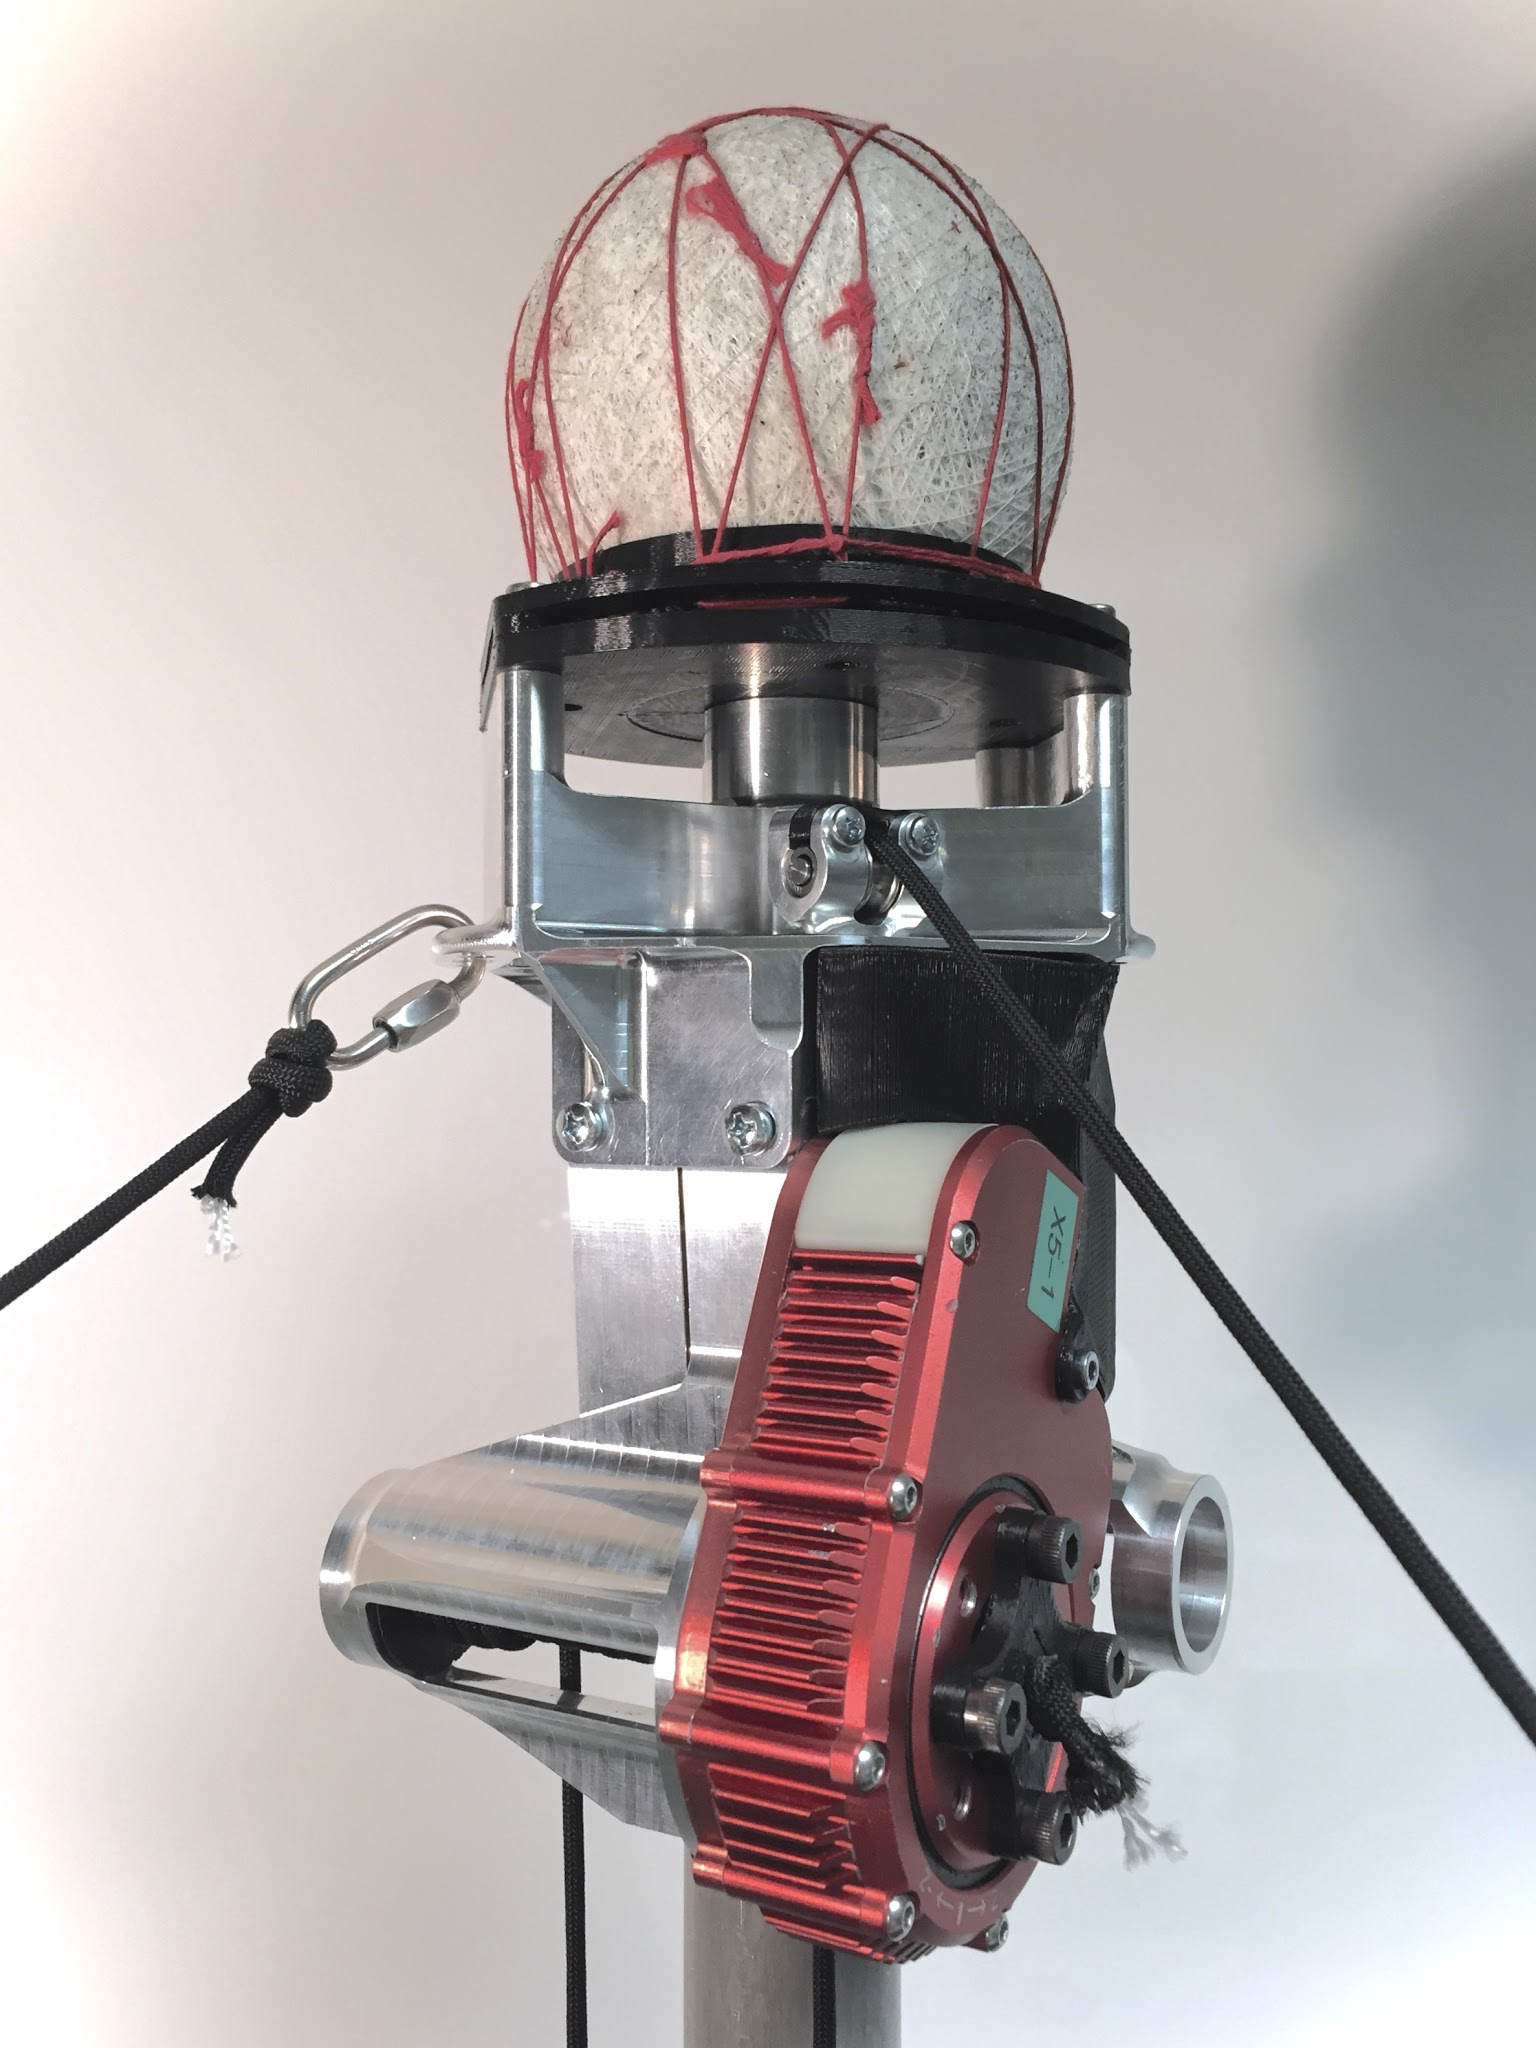
\includegraphics[width=.8\linewidth]{tex/img/sb_v2_close}
  \caption{}
  \label{fig:sbv2_close}
\end{subfigure}%
\begin{subfigure}{.5\textwidth}
  \centering
  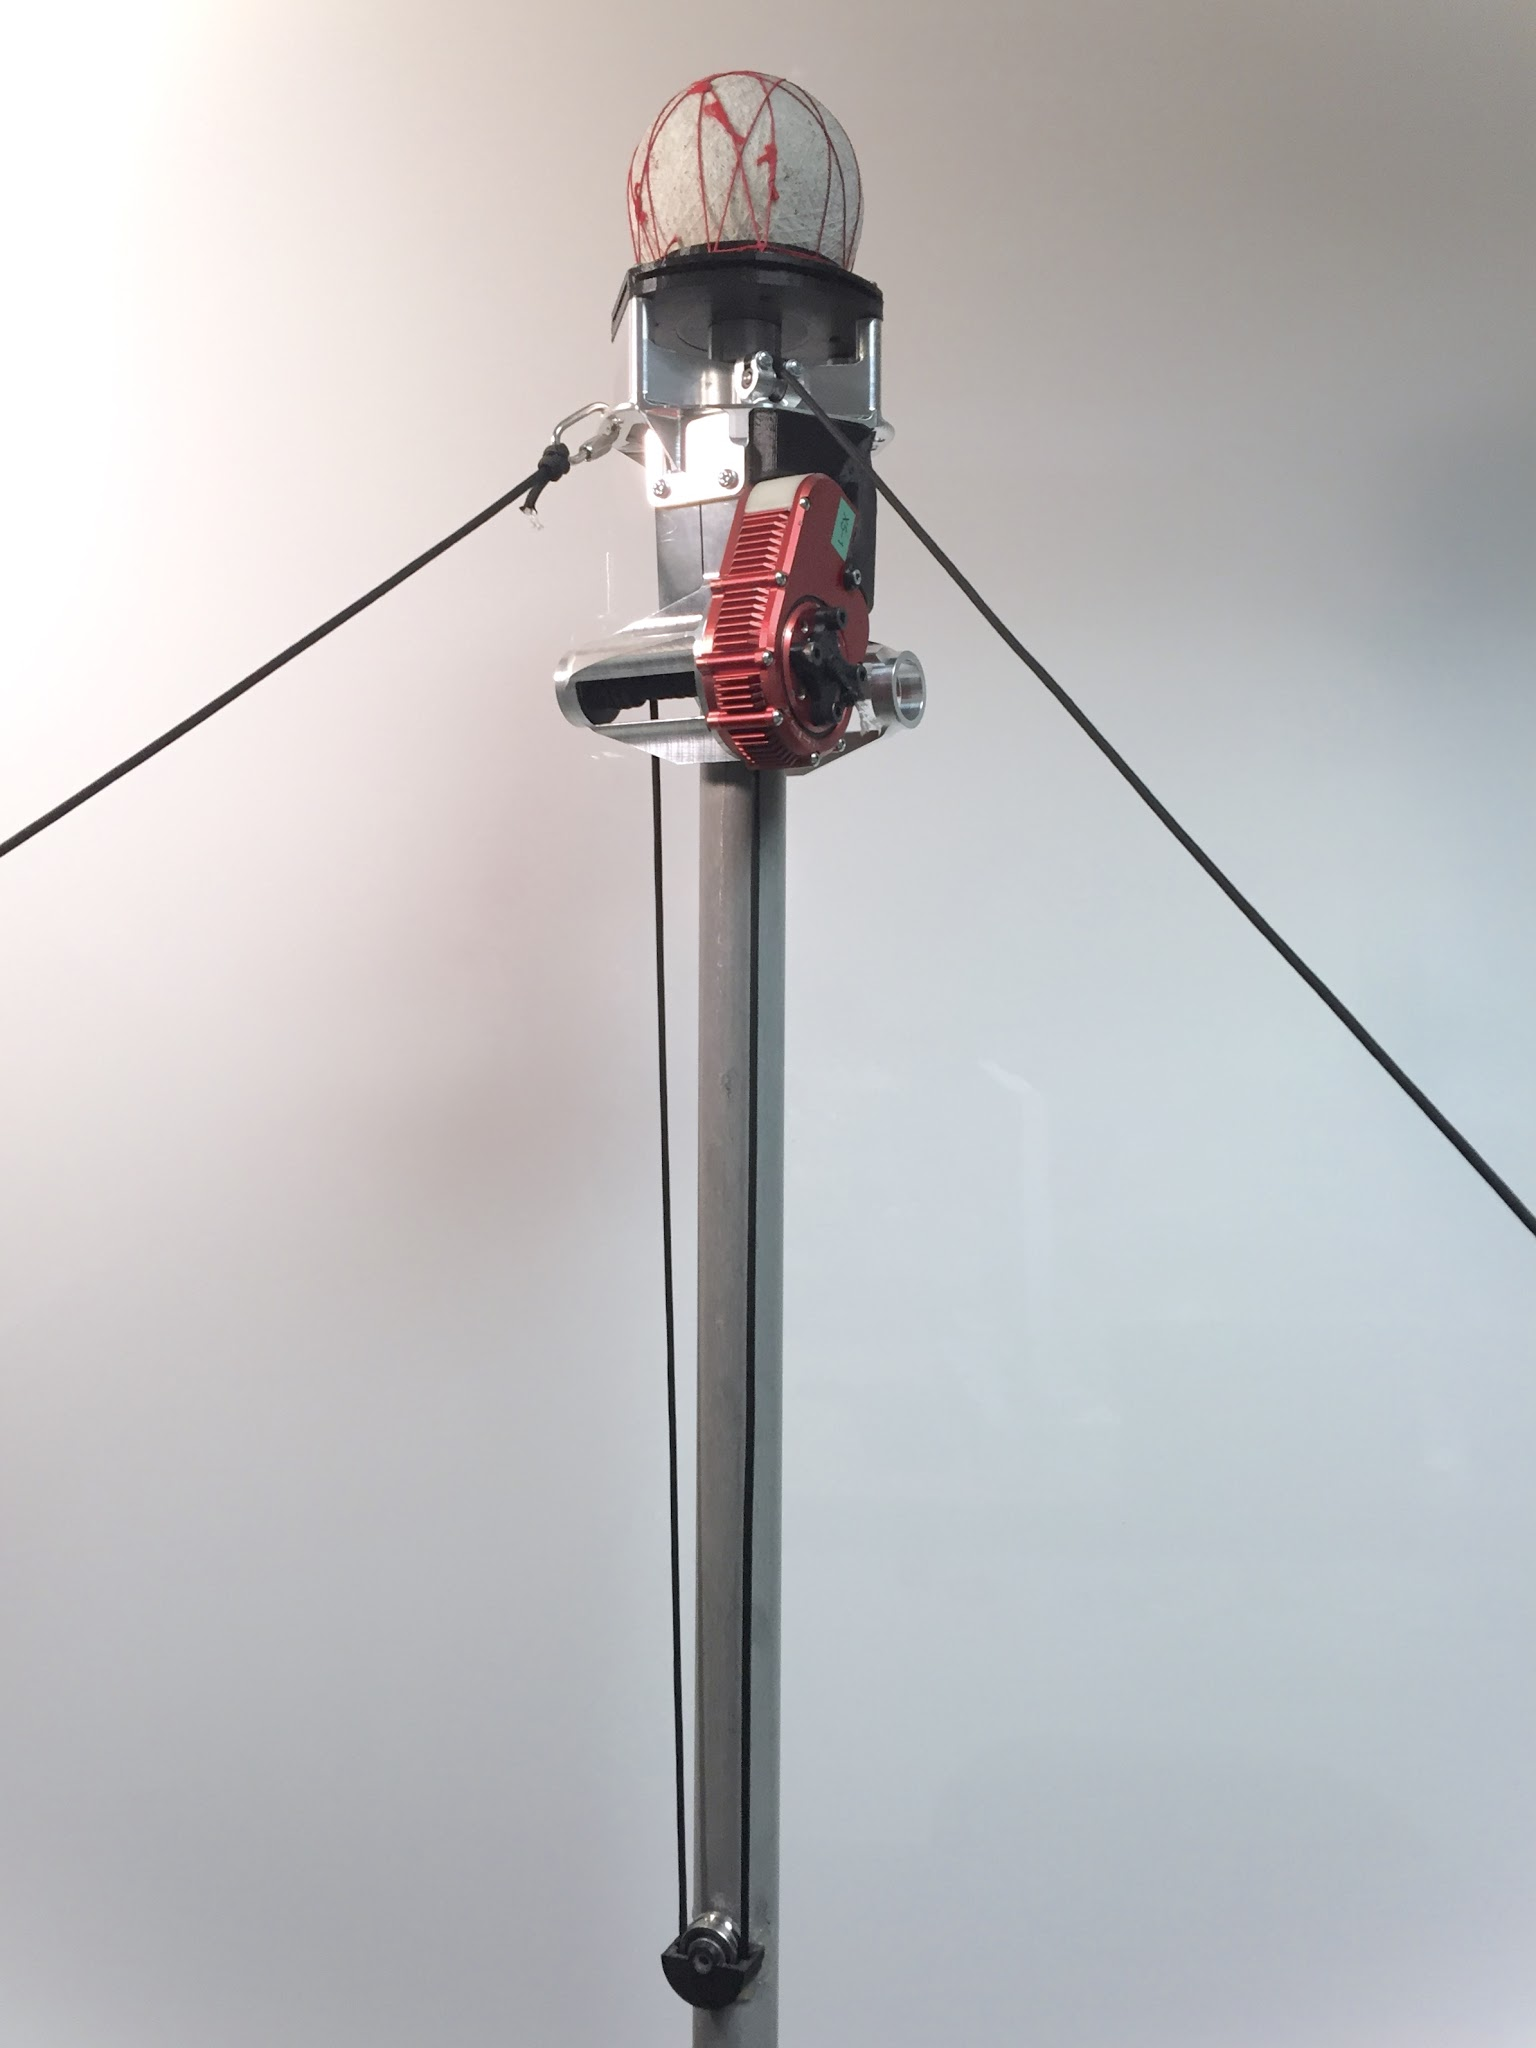
\includegraphics[width=.8\linewidth]{tex/img/sb_v2_far}
  \caption{}
  \label{fig:sbv2_far}
\end{subfigure}
\caption{Images of initial \SB{} v2 MTR designs. (a) Close up of initial design for \SB{} v2. An omni directional cable guide can be seen which eliminates cable friction. (b) Full cable routing where the cable is run over a distal pulley to increase cable length for a better effective spring constant induced by the cable stretch.}
\label{fig:sbv2}
\end{figure}

% Please add the following required packages to your document preamble:
% \usepackage[table,xcdraw]{xcolor}
% If you use beamer only pass "xcolor=table" option, i.e. \documentclass[xcolor=table]{beamer}
\begin{table}[tbhp]
\centering
\caption{Comparison between the current \SB{} v1 and the intended design of \SB{} v2}
\label{sb_versions_compare}
\resizebox{\textwidth}{!}{%
\begin{tabular}{|
>{\columncolor[HTML]{FFFFFF}}c |
>{\columncolor[HTML]{EFEFEF}}c |
>{\columncolor[HTML]{FFFFFF}}c |
>{\columncolor[HTML]{EFEFEF}}l |
>{\columncolor[HTML]{FFFFFF}}l |
>{\columncolor[HTML]{EFEFEF}}c |}
\hline
\textbf{}                                                      & \cellcolor[HTML]{EFEFEF}\textbf{\begin{tabular}[c]{@{}c@{}}Number of\\ Actuators\end{tabular}} & \textbf{Size / Weight} & \multicolumn{1}{c|}{\cellcolor[HTML]{EFEFEF}\textbf{Motor Controls}} & \multicolumn{1}{c|}{\cellcolor[HTML]{FFFFFF}\textbf{Sensors}}                                                                       & \textbf{\begin{tabular}[c]{@{}c@{}}Maximum Length for\\ Change in Cable Length*\end{tabular}} \\ \hline
\textbf{\begin{tabular}[c]{@{}c@{}}\SB{} \\ v1\end{tabular}} & \cellcolor[HTML]{EFEFEF}12                                                                     & \(\SI{1.75}{\meter} \text{/} \SI{21}{\kilo\gram}\)                      & \cellcolor[HTML]{EFEFEF}Position                                     & \begin{tabular}[c]{@{}l@{}}Motor Encoders\\ Accelerometer, Gyro, Magnetometer \\ Ranging / localization Sensors\end{tabular}        & \(\SI{0.4}{\meter}\)                                                                                             \\ \hline
\textbf{\begin{tabular}[c]{@{}c@{}}\SB{} \\ v2\end{tabular}} & 24                                                                                             & \(\SI{1.8}{\meter} \text{/} \SI{30}{\kilo\gram}\)                      & \begin{tabular}[c]{@{}l@{}}Position\\ Velocity\\ Torque\end{tabular} & \begin{tabular}[c]{@{}l@{}}Motor Encoders\\ Motor Torque Sensor\\ Accelerometer, Gyro\\ Ranging / localization Sensors\\ Linear Cable Sensors\end{tabular} & \(\SI{1.5}{\meter}\)                                                                                             \\ \hline
\end{tabular}
}
\raggedright{\footnotesize * This is the total length a single motor can pull starting with no cable wound on the spool. For \SB{} v2 this means the start length of cable will mean the robot will be in a collapsed state initially.}
\end{table}

The redesign of \SB{} is still in very early stages of development, however table~\ref{sb_versions_compare} shows some of the differences in base physical properties and features between the two versions.

\subsection{Extending Controls for a Fully Actuated \SB{} v2}
\label{sec:future_controls}

In chapter~\ref{controls}, there was a focus on learning a forward locomotion gait for a hardware system that had very limited actuation.
\SB{} v2 aims to address these limitations and expand the robustness of the system, which will open up new areas of research.
This system will allow for forward locomotion to be achieved through the "basic" gait as outlined in section~\ref{basic_locomotion}.
Using this control method as well as the basic steering from section~\ref{sec:steering} as priors for the learning method outlined in section~\ref{sec:mdgps}, highly optimized gaits for navigation should be rapidly achieved.

\subsubsection{Decentralized Control}
One limitation with the controllers developed so far for \SB{} is their reliance on centralized controllers for basic locomotion.
A computer connects to \SB{}'s network in order to receive and send data over a standard 802.11~\cite{ieee1997wireless} wireless protocol using the ROS UDP messaging protocol.
This allows for easy communication between the robot and the control computer, however large amounts of data can be lost from this network structure.
High data loss dramatically affects the performance of a controller and may even cause the controller to fail.
Utilizing a decentralized control method will allow the individual actuators to adapt without this wireless network layer.
Mirletz \etal developed a control scheme which uses a Central Pattern Generator on each actuator to achieve decentralized locomotion for a snake like tensgerity structure~\cite{mirletz2015goal}.
Taking this approach and replacing the learning method with the guided policy search method shown in section~\ref{sec:mdgps}, a controller could be learned in a fraction of the time that may require no hand tuning to implement on hardware.
This will enable \SB{} to learn gaits optimized for various terrains which requires no external centralized control input.

\subsubsection{Path Planning}
Having basic locomotion controls achieved, high level navigation and path planning techniques can be researched and demonstrated.
The path planning method discussed in section~\ref{sec:belief}, currently relies on random actuator commands to actuate the simulated \SB{} like robot along a given path.
The author directly states that faster and more computationally efficient paths will be generated if the algorithm can assume some level of confidence when selecting a control input~\cite{littlefieldintegrating}.
Using a method like the guided policy search method mentioned above, a list of control inputs for various scenarios may be compiled.
It may also be possible to integrate the GPS algorithm into the path planning method, enabling the creation of efficient gaits when new environments are encountered.

\section{Conclusion}

This works hopes to inform and further future research into tensegrity and highly compliant cable driven robotics, and their applications in terrestrial exploration.
The future of terrestrial robotics will utilize passive compliance to adapt and perform in scenarios such as rocky and icy terrain, surviving high falls, and navigating through extreme conditions where it will be difficult for non-passively compliant robots to perform.

% \begin{itemize}
% % \item Building of \SB{} v2
% % \item With \SB{} v2, control methods using 24 actuation will be implemented on hardware
% % \item Use Guided Policy Search algorithm to learn CPG parameters for rolling and other manuvering tasks
% % \item Combine state estimation with locomotion tasks to implement Belief Space motion planning
% \item Use machine learning techniques to find "packing" controllers
% \end{itemize}


% \color{red}
% \section{Current Prototype's Limitations and Possible Design Changes}


% \section{Utilizing Locomotion Controllers to Enable High Level Trajectory Planning}


% \color{blue}
% TODO: Most of the text below will be moved to other sections or deleted 

% \section{\SB{} Current State}
% At this point, the first goal proposed in section \ref{goal} has been achieved.
% \SB{} is composed of twelve Modular Tensegrity Robots (MTR) attached as the ends of 6 rods connected in a icosahedron geometry, and may be seen in figure \ref{fig:SB}.
% Preliminary testing of the system, presented in the following sections, has shown many of the basic functions and features that will enable goals two and three.
% All data collected in this section was collected through the wireless ROS network with no extra sensors or equipement apart from what was designed into the system, explained in chapter \ref{design}. 

% \section{Future Work}

%\subsection{Proposed Controls Methods}

% \subsection{Open Loop Locomotion Control}
% \label{open_loop}
% For clarity, open loop used here is open in regards to the locomotion system's ability to change robotic motor inputs based on environmental sensing.
% Work presented in~\cite{iscen2014flop} shows through simulation that a tensegrity system like \SB{} can achieve a rolling gait by deforming the triangle currently in contact with the ground.
% Though \SB{} is not fully actuated (all 24 external cables are attached to motors), a derivative of this work may be able to be applied to \SB{}.
% Leveraging the experimental results from section \ref{basic_locomotion}, \SB{} can achieve open loop locomotion quite easily with the addition of detecting which face of the robot is on the ground.
% To achieve this ground detection, I propose to use the IMU modules on each sensor board to detect earth's gravity field and/or ground contacts when a rod contacts the ground.
% Using a basic machine learning technique, like k-nearest neighbor, may enable successful classification of where the ground is in relation to the robot.

% \subsection{Closed Loop Locomotion Control}
% There has been preliminary results done by~\cite{burms2015online} which demonstrates a tensegrity robot sensing different enviromental terrains.
% This shows promise that a tensegrity robot may sense changes in terrain without the need for extra sensors.
% If a similar technique can be achieved on \SB{} in a real-time manor, then the open loop gait pattern used from \ref{open_loop} can be altered to better locomote over the sensed terrain.
% This new locomotion gait may either be hand tuned parameters or learned behavior.
